% VLDB template version of 2020-08-03 enhances the ACM template, version 1.7.0:
% https://www.acm.org/publications/proceedings-template
% The ACM Latex guide provides further information about the ACM template

\documentclass[sigconf, nonacm]{acmart}
\usepackage{pgfplots}


\usepackage{algorithm2e}
\usepackage{multicol}
%% The following content must be adapted for the final version
% paper-specific
\newcommand\vldbdoi{XX.XX/XXX.XX}
\newcommand\vldbpages{XXX-XXX}
% issue-specific
\newcommand\vldbvolume{14}
\newcommand\vldbissue{1}
\newcommand\vldbyear{2020}
% should be fine as it is
\newcommand\vldbauthor{\author} 
\newcommand\vldbtitle{\shorttitle} 
% leave empty if no availability url should be set
\newcommand\vldbavailabilityurl{http://vldb.org/pvldb/format_vol14.html}
% whether page numbers should be shown or not, use 'plain' for review versions, 'empty' for camera ready
\newcommand\vldbpagestyle{plain} 

\begin{document}
\title{Adversarial Attacks on self driving cars using adversarial patches on road signs}

%%
%% The "author" command and its associated commands are used to define the authors and their affiliations.


\author{Miryam Kayali}
\affiliation{%
  \institution{American University of Beirut}
  \city{ }
  \country{ }
}
\affiliation{%
  \institution{Computer Science}
  \city{Beirut}
  \country{Lebanon}
}
\email{mmk97@mail.aub.edu}

\author{Marina Kayrouz}
\affiliation{%
  \institution{American University of Beirut}
  \city{ }
  \country{ }
}
\affiliation{%
  \institution{Computer Science}
  \city{Beirut}
  \country{Lebanon}
}
\email{mhk46@mail.aub.edu}


\author{Hani Alsabe}
\affiliation{%
  \institution{American University of Beirut}
  \city{ }
  \country{ }
}
\affiliation{%
  \institution{Computer Science}
  \city{Beirut}
  \country{Lebanon}
}
\email{hma115@mail.aub.edu}


\author{Mohamed El Baker Nassar}
\affiliation{%
  \institution{American University of Beirut}
  \city{ }
  \country{ }
}
\affiliation{%
  \institution{Computer Science}
  \city{Beirut}
  \country{Lebanon}
}
\email{mn115@mail.aub.edu}


%%
%% The abstract is a short summary of the work to be presented in the
%% article.
\begin{abstract}
Recent studies show that attacking an object detector is more difficult than attacking an image classifier, as it needs to mislead the classification results in multiple bounding boxes with different scales. Extending the digital attack to the physical world adds another layer of difficulty because it requires the perturbation to be robust enough to survive real-world distortions due to different viewing distances and angles, lighting conditions, and camera limitations. In this report, we will be discussing classifiers and detectors that can generate an adversarial perturbed stop signs that are consistently mislead as other objects, posing a potential threat to autonomous vehicles and other safety-critical computer vision systems. Moreover, we will propose an evaluation of the performance, including some of their implementation, of the classifiers and detectors we discussed.

\end{abstract}

\maketitle



\section{Introduction}

The recognition of traffic signs has received increasing attention in recent years. Self-driving cars need traffic sign recognition in order to properly parse and understand the roadway. Similarly, “driver alert” systems inside cars need to understand the roadway around them to help aid and protect drivers. Traffic sign classification is the process of automatically recognizing traffic signs along the road, including speed limit signs, yield signs, merge signs, etc. Being able to automatically recognize traffic signs enables us to build “smarter cars”. Traffic sign recognition is just one of the problems that computer vision and deep learning can solve. We first detect that this object is a traffic sign then classify it. In this project we study traffic sign object detection and classification. We then survey adversarial attacks against traffic sign detection and classification. 

\section{ General Object Detection and classification }
% In this section, a brief summary about the difference between classification and detection process will be mentioned. The upcoming section discussed the related work that belongs to phase 1. Then, section 2.2 talks about the related work that we rely at for building the proposed solution.

\subsection{Dataset and Classifiers}
The algorithm has two steps: we first detect then classify. The detection benchmark is a process of actually finding out about item features The classification benchmark task is a process of putting items into different bins. For example, in the GTSRB detection benchmark task, the algorithms must detect traffic signs in one of four major categories. In the GTSRB classification benchmark, the traffic sign occupies most of the image, and the algorithms must only decide which subclass the class belongs to. There exist  multiple detectors and classifiers, but we will focus on the following . LISA-CNN is a classifier that uses LISA dataset, a U.S. traffic sign dataset containing 47 different road signs. We also have GTSRB-CNN which uses German Traffic Sign Recognition Benchmark (GTSRB). On the other hand, Faster R-CNN is a detector that uses Microsoft COCO benchmark. Another competitor is the chinese version of R-CNN that also uses Microsoft COCO dataset\cite{Abril03}. And finally, the newest detector is Retinanet\cite{Abril01}, a two-stage framework that consistently achieves top accuracy on the challenging COCO benchmark. We will be explaining the difference between a detector and a classifier in the following section.

\begin{table}[hb]% h asks to places the floating element [h]ere.
  \caption{Detectors and Classifier}
  \label{tab:freq}
  \begin{tabular}{ccl}
    \toprule
    Networks & Type & Dataset\\
    \midrule
    GTSRB-CNN &  Classifier & GTSRB\\
    LISA-CNN & Classifier & LISA\\
    Faster R-CNN & Detector & Microsoft COCO\\
    R-CNN (Chinese version) & Detector & Microsoft COCO\\
    Retinanet & Detector & Microsoft COCO\\
  \bottomrule
\end{tabular}
\end{table}



\subsection{ Traffic sign detection and classification 
}
Traffic-sign recognition is divided into a two-phase task: detection followed by classification. People often confuse image classification and object detection. The detection phase uses shared data to build bounding boxes that may contain traffic-signs in other words it is the process of actually finding out about the object features, whereas the classification phase uses differences to label the kind of sign shown if present. In other words, every detector is a classifier but not every classifier is a detector. 
Recently, convolutional neural networks, that are based on a two-staged approach popularized by R-CNN, have been shown to outperform such simple classifiers like Lisa and GTSRB. Although GTSRB and LISA have a high precision rate with 95.7\% and 91\% respectively, these approaches perform classification on already detected signs, which is impractical in real applications. Detectors are more challenging to attack since the adversarial examples need  to not only mislead the label predictions but also the existence of the object. 

\subsection{ Comparison between detectors}
Convolutional Neural Networks (CNN) have come a long way in conveniently identifying objects in images and videos. Networks like Yolov3, R-FCN, SSD, Fast RCNN, and Fast RCNN - Chinese and many more have evolved over time. Object detectors that are based on a two-stage approach are said to have the highest accuracy. Two-stage detector does not just use a sliding window detection. Instead, the system consists of two components: the first component  is object proposal components and second component is to classify the sparse set of proposals. In contrast, One-stage detectors  run a similar sliding window detection on a densely populated tree. One-stage detectors have the potential to be faster and simpler, but have trailed the accuracy of two-stage detectors thus far. This detector obtains a better performance when it has more bounding boxes to better cover the space of possible objects. Therefore, is it found that the accuracy can be recovered by densely covering the space of all the possible locations that could contain objects. Therefore a recent study, Focal Loss for Dense Object Detection, showed that one-stage detector can out perform a two-stage detector by reshaping the standard cross entropy loss such that it down-weights the loss assigned to well-classified examples. Creating a one-stage detector, called RetinaNet\cite{Abril01}, that showed to match the speed of a one-stage detectors while outperforming the accuracy of a two-stage detectors.
According to their results, on Microsoft COCO dataset, the two Convolutional Neural Networks that has the highest accuracy is RetinaNet and Faster R-CNN* with a 40.8\% and 34.9\% mAP respectively. Faster R-CNN has an average mAP of 21.9\% . R-FCN has mAP of 31.5\% . SSD300 and SSD512 have mAPs of 23.2 and 26.8 respectively . YOLO-V2 is at 21.6\% whereas YOLO-V3 is at 33\% . FPN delivers 33.9\% 


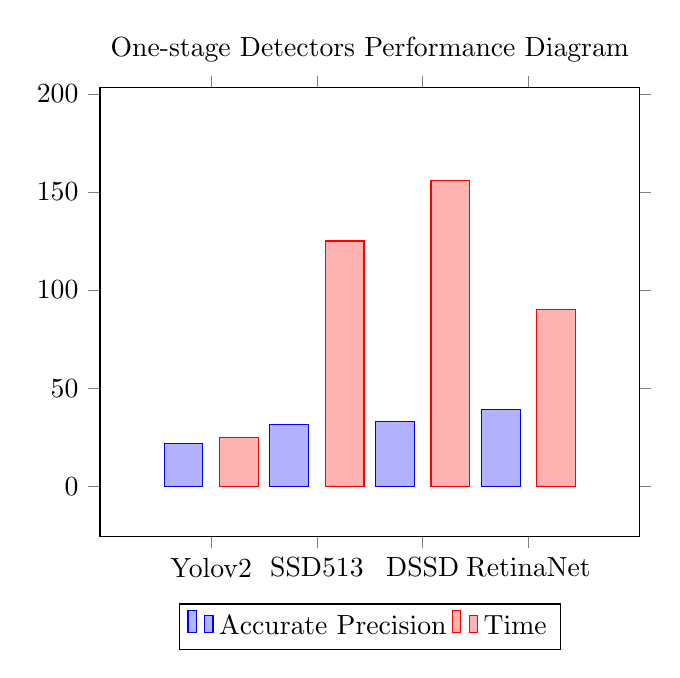
\begin{tikzpicture}
\centering
\begin{axis}[
	%x tick label style={
	%	/pgf/number format/1000 sep=}, 
    title  = One-stage Detectors Performance Diagram,
    xbar,    
% 	ylabel=Quality,
    y label style={at={(0.07,0.5)}},
	enlargelimits=0.35,  %%zoom in or out
    %legend style={at={(0,0)},
	legend style={at={(0.5,-0.15)},
	anchor=north,legend columns=-1},
	%ybar interval=0.7,
    ybar=6pt,
    bar width=14pt,
    symbolic x coords={Yolov2,SSD513,DSSD,RetinaNet},
    xtick=data]
]
\addplot 
	coordinates {	(RetinaNet,39.1) (DSSD,33.2) (SSD513,31.5)
		 (Yolov2,21.6)  };
\addplot 
	coordinates {	(RetinaNet,90) (DSSD,156) (SSD513,125) 
		(Yolov2,25)  };
\legend{Accurate Precision,Time}
\end{axis}
\end{tikzpicture}
\newline \\\\ \\\\
    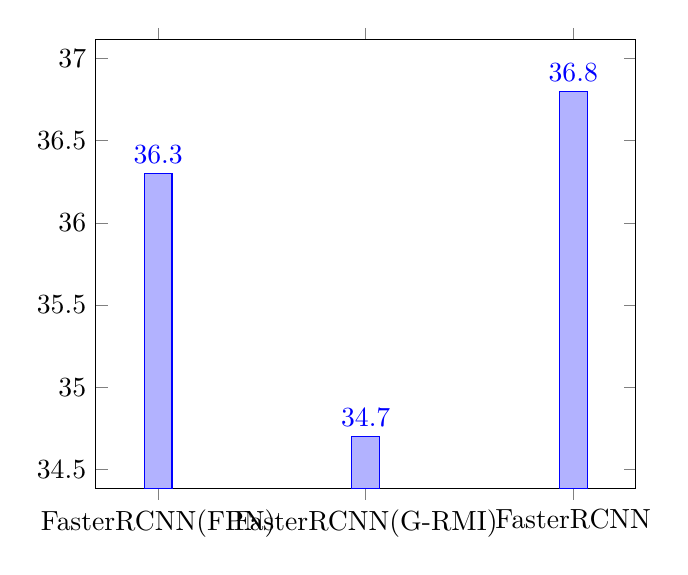
\begin{tikzpicture}
\begin{axis}[
    ybar,
    enlargelimits=0.15,
    legend style={at={(0.5,-0.15)},
      anchor=north,legend columns=-1},
    symbolic x coords={FasterRCNN(FPN),FasterRCNN(G-RMI),FasterRCNN},
    xtick=data,
    nodes near coords,
    nodes near coords align={vertical},
    ]
\addplot coordinates {(FasterRCNN(FPN),36.3) (FasterRCNN(G-RMI),34.7) (FasterRCNN,36.8)};
\end{axis}
\end{tikzpicture}





Their results  showed a 5.9 point AP gap  (39.1 vs. 33.2) between RetinaNet and it’s one-stage competitor, DSSD , while also being faster, as shown in the table above. One the other hand, RetinaNet achieves a 2.3 point gap above the top-performing two-staged detector, Faster R-CNN model, based on Inception-ResNet-v2-TDM.

\section{Transfer learning}
Transfer learning is one of the methods of training machine learning algorithms. It is a popular approach in deep learning for speeding up the training step and improving the performance, given the vast computation and time required to develop neural network models. It works by storing the knowledge it gained while solving one problem and using this knowledge for another related task. For instance, if we want to train a convolutional neural network image classifier to identify an object (e.g stop signs) and we only have 1000 images of stop signs. This is not enough to train the model so we can use an existing pre-trained CNN model (e.g ResNet model) and this model is trained with millions of traffic signs so it already understands how traffic signs look like. Over that the model can be trained on the 1000 stop sign images. So the pre-trained model gets more training specifically on the stop signs and thus this model can recognize stop signs very well compared to the model which we might try to train it only with 1000 images. Using this methodology, we will be using ResNet50 as our pre-trained model and then feed it our data set on traffic signs to train on it.
\section{Attacks}
\subsection{Theoretical models of the attacks (math) }
\subsubsection{ Robust Physical Perturbations (RP2) }
The algorithm starts with an optimization method that generates a perturbation for a single image x, with considering other physical conditions. This single-image optimization problem is solved with Lagrangian-relaxed formula\cite{Abril07}. 

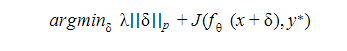
\includegraphics[scale=0.75]{file 1.png}

\\Here J(· , ·) is the loss function, which measures the difference between the model’s prediction and the target label y* . $\lambda $ is a hyper-parameter that controls the regularization of the distortion. We specify the distance function H as ||$\delta$||p, denoting the lp norm of $\delta$.

Next, the objective function was modified to account for the physical conditions. They did that by modeling  the distribution of images containing object o (e.g stop sign) under both physical and digital transformations X$^v$. Different sampling instances xi were taken from X$^v$ by both generating experimental data that contains actual physical condition variability as well as synthetic transformations (e.g changing distances, angles, and lightning). For synthetic variations, the object is cropped randomly within the image, change in brightness, and an addition of spatial transformations was done to simulate other possible conditions. A mask was introduced to ensure that the perturbations are only applied to the surface area of the target object o. Several masks were done as graffiti or stickers  to generate perturbations that are visible but inconspicuous to human observers. Formally, the perturbation mask is a matrix Mx whose dimensions are the same as the size of input to the road sign classifier. Mx contains zeros in regions where no perturbation is added, and ones in regions where the perturbation is added during optimization.
The fabrication error problem was solved, by using Non-Printability Score (NPS) by Sharif et al, to the objective function that models printer color reproduction errors. Given a set of printable colors (RGB triples) P and a set R($\lambda$) of (unique) RGB triples used in the perturbation that need to be printed out in physical world, the non-printability score is given by:

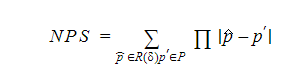
\includegraphics[scale=0.60]{file2.png}

The NPS formula was used to generate the following final robust spatially constrained perturbation: 
\\
\\

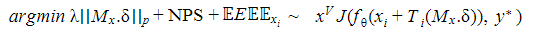
\includegraphics[scale=0.60]{file3.png}

The function Ti(.) is used to denote the alignment function that maps transformations on the object to transformations on the perturbation (e.g. if the object is rotated, the perturbation is rotated as well). Finally, an attacker will print out the optimization result on paper, cut out the perturbation (Mx), and put it onto the target object o.

\subsubsection{ Shapeshifter }

Shapeshifter is a white-box attack; this means that it can compute outputs and gradients since it has access to the model structure.\cite{Abril07} The Shapeshifter method was adopted from the Change-of-variable method and Expectation over Transformation. 
\\Change-of-variable method: 
\\Denote LF (x, y) = L(F (x), y) as the loss function that calculates the distance between the model output F (x) and the target label y. Given an original input image x and a target class y.
\\
\\
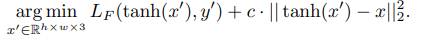
\includegraphics[scale=0.60]{file9.png}
\\
\\
The use of tanh ensures that each pixel is between [−1, 1]. The constant c controls the similarity between the modified object x' and the original image x.
\\Expectation over Transformation method: 
\\This method adds random distortions in each iteration of the optimization to make the perturbations more robust. Given a transformation t that can be translation, rotation, and scaling, Mt(xb, xo) is an operation that transforms an object image xo using t and then overlays it onto a background image xb. After adding the random distortions the method becomes as the following: 
\\
\\
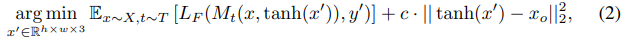
\includegraphics[scale=0.60]{file8.png}
\\
\\
where X is the training set of background images. 
Formation of Shapeshifter method: 
As we mentioned earlier, Fast RCNN is a two-stage detector. The first stage finds several regions of interest, and the second stage performs classification within each of the detected regions. Let rpn(x) = {r1,...,rm}, where each ri is a detected region represented as its four coordinates, and let xr be a sub-image covered by region r. Denote LFi(x,y) = L(F (xri ), y) the loss of the classification in the i-th detected region. We simultaneously attack all the classifications in each region by the following optimization.\cite{Abril07}
\\
\\
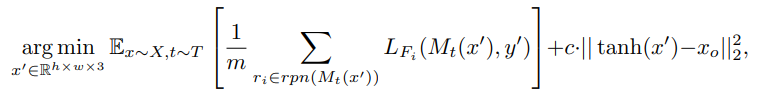
\includegraphics[scale=0.40]{file11.png}
\\
  

\subsection{ Most successful attacks against stop signs  }
Early researches mainly focused on studying adversarial examples against the image classifiers in the physical world. An attack called Robust Physical Perturbations (RP2)\cite{Abril02} was made in April 2018 on two classifiers LISA\_CNN and GTSRB\_CNN to fool self-driving cars when detecting traffic signs (e.g stop signs), They showed that it is possible to generate physical adversarial examples robust to the physical environmental challenges and widely varying distances/angles.\cite{Abril07} The three types of adversarial examples that were made on these classifiers were object constrained poster printing, sticker, and camouflage-art. High attack success rate was observed for all types. Table 1 summarizes a sampling of stationary attack images from different angles and distances and their success percentage.
\\
\\
  \begin{tabular}{ccl}
    \toprule
    Type & Targeted-Attack Success\\
    \midrule
    Subtle Poster &  100$\%$ \\
    Camouflage Graffiti & 66.67$\%$\\
    Camouflage Art (LISA-CNN) & 100$\%$\\
    Camouflage Art (GTSRB-CNN) & 80$\%$\\
  \bottomrule
\end{tabular}
\\
\\
\\Table 1: Sample of physical adversarial examples against LISA-CNN and GTSRB-CNN.
\\
\\Until very recently, there have been a few studies attacking object detectors in the physical space. In July 20 2018, a stronger modified version of RP2 was made that targeted detectors rather than just classifiers. The results of their adversarial examples showed that they are robust in the real world environment and capable of attacking the state-of-the-art object detectors such as YOLO v3 and Faster-RCNN. Their results showed that our adversarial poster perturbation fools YOLO v2 in 85.6\% of the video frames recorded in an indoor lab environment and in 72.5\% of the video frames recorded in an outdoor environment. Also their adversarial stickers fool YOLO v2 in 85\% of the video frames recorded in a laboratory environment and in 63.5\% of the video frames recorded in an outdoor environment. As for the results on Faster R-CNN, the success fool rate was 85.9\% in the video frames recorded in a laboratory environment and 40.2\% in the video frames recorded in an outdoor environment.After that in February 2019, another adversarial attack was done on the chinese version of RetinaNet and on YOLO, called Daedalus\cite{Abril03}. Robust Daedalus examples were generated by using an ensemble of popular backbone networks as the substitutes can launch the attack in a black-box scenario. But these attacks focus on the general approach of the object detectors and are not specific to road signs.
\\In May 2019, another adversarial attack was done on Faster R-CNN, called ShapeShifter\cite{Abril07}. The object detector Faster R-CNN adopts a two stage detection strategy. First, using a region proposal network it generates several class-agnostic bounding boxes called region proposals that may contain objects. Second, using a classifier and a regressor it outputs the classification results and refined bounding box coordinates for each region proposal, respectively. The computation cost is significantly reduced by sharing the convolutional layers in the two stages. Faster R-CNN is considered robust to physical adversarial attacks since a single object can be covered by multiple region proposals of different sizes and aspect ratios, and one needs to mislead the classification results in all the region proposals to fool the detection. The adversarial attack is generated by performing the optimization process described above. The perturbation strength is determined by the hyperparameter c, the smaller c is, the more conspicuous the perturbation. But, getting a robust attack means using a very small c, which leads to having a road sign that is difficult to be categorized by the human eye.  So when building the attack on a stop sign, the perturbation focuses only on the red part of the sign leaving the white text intact. Which leads to a robust perturbation and having enough contrast between the red parts and the lettering so a human can recognize it easily. Shapeshifter can perform two targeted attacks (person and sports ball) and one untargeted attack. Having said that, Shapeshifter achieves a high attack success rate in misleading the object detector at different angles and distances. These results are summarized in  Table 2. 
\begin{table}[hb]% h asks to places the floating element [h]ere.
  \label{tab:freq}
  \begin{tabular}{ccl}
    \toprule
    Type & Targeted & Untargeted\\
    \midrule
    Person & 87 $\%$ & 93 $\%$ \\
    Sport Ball & 40$\%$ & 93 $\%$\\
    Untargeted & N/A & 73$\%$\\
  \bottomrule
\end{tabular}
\end{table}
\\
\\Table 2: Targeted - Attack success rate for different categorize against stop signs. 
\\
These results show that high-confidence perturbations achieved at a high attack success rate at a variety of distances and angles. The untargeted attack can mislead the detection into a clock. 
Our work demonstrates vulnerability in MS-COCO-learned object detectors and posits that security and safety critical systems need to account for the potential threat of adversarial inputs to object detection systems.
\section{Results}
We performed a digital attack on retinanet using adversarial images that was generated by Shapeshifter. The retinanet version that we are using was not built to detect road signs, but objects in general. By changing the dataset in the code, we achieved a detection on  a simple road sign image of 0.562 inference. Image 1 shows the results. \\
\\
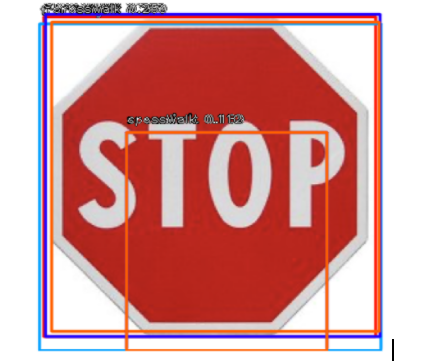
\includegraphics[scale=0.40]{stop sign.png}
\\
Image 1: Stop sign detection by RetinaNet-101-800 model
\\
When we tried to detect an adversarial image taken from Shapeshifter results using RetinaNet. The digital attack performed on Shapeshifter detected a road sign as a person with 70 percent accuracy. The RetinaNet-101-800 model didn’t detect it. When trying to detect other adversarial images using RetinaNet, they were not detected. All the adversarial images were not detected by the RetinaNet-101-800 model.  
On another hand, we tested the accuracy of the adversarial images generated by RP2 using google image classification. All the images were not classified as a road sign image but as different categories. Some were classified as a photographer (person) with a maximum of 96$\%$ accuracy, or as colors with a maximum of 94$\%$ accuracy and many more. Table 3 shows the different results. 
\begin{table}[hb]% h asks to places the floating element [h]ere.
  \label{tab:freq}
  \begin{tabular}{ccl}
    \toprule
    Tags & Maximum accuracy \\
    \midrule
    Person (photograph) & 96$\%$ \\
    Toy & 56$\%$ \\
    Colors & 99$\%$ \\
    Clock & 55$\%$ \\
    Baked Goods & 55$\%$ \\
    Lighting & 57$\%$ \\
    Food & 50$\%$
  \bottomrule
\end{tabular}
\end{table}
\\
\\Table 3:  Different classifications results using google image classification with RP2 adversarial attack on LISA-CNN
\\
The different results can be tested using our codes found in our github repository and can be found on our website. 
\section{Contribution}
\begin{itemize}
  \item Modified the dataset in the RetinaNet-101-800 model to detect road sign images. 
  \item Attacking the RetinaNet-101-800 model by running an adversarial image generated by Shapeshifter showed no results. Which means that RetinaNet-101-800 model can be attacked using a similar approach than Shapeshifter.
  \item Similarly, using RP2 adversarial images, google image classification was fooled and misclassified the road sign image. 
    \item All the codes used in these detectors and adversarial attacks can be found in our github repository. Due to having old versions of the different detectors and attacks, these can only work on old versions of tensorflow and python 2. In our repository, we have uploaded different codes and updated the dependencies to have a working code.
    \item Finally, to further show the difference between the two adversarial attacks on Lisa-CNN and Faster R-CNN, we made a website showing both adversarial attacks on road signs. Shapeshifter can mislead the detector into classifying a road sign into 90 different tags. We choose to display only 5 different tags. Similarly, RP2 can mislead a detector into classifying a road sign as 7 different tags, we choose to show 5.
\end{itemize}
\section{Future Work}
The RetinaNet-101-800 model achieved top results, outperforming both one-stage and two-stage models like Faster R-CNN and YOLO. Until now, there has been no successful  attack on the RetinaNet-101-800 model. In the future, an adversarial attack on the RetinaNet-101-800 model can be done by combining the two approaches used in ShapeShifter and RP2. 

% \begin{figure}
%   \centering
%   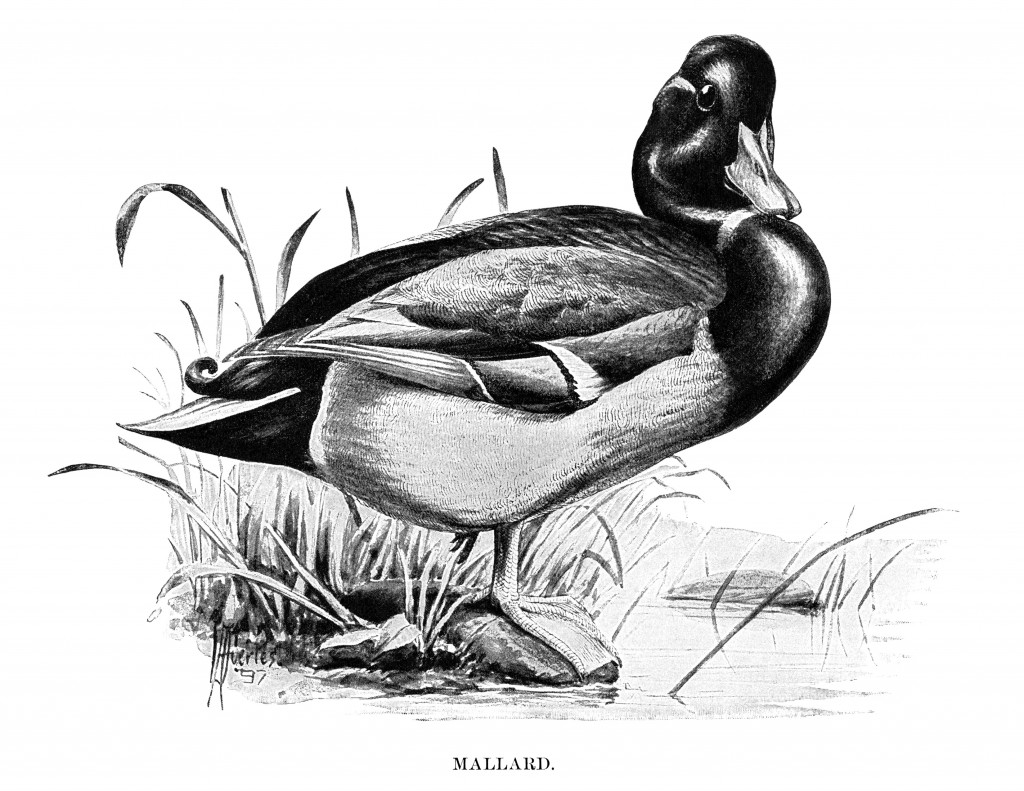
\includegraphics[width=\linewidth]{figures/duck}
%   \caption{An illustration of a Mallard Duck. Picture from Mabel Osgood Wright, \textit{Birdcraft}, published 1897.}
%   \label{fig:duck}
% \end{figure}

% \begin{table*}[t]
%   \caption{A double column table.}
%   \label{tab:commands}
%   \begin{tabular}{ccl}
%     \toprule
%     A Wide Command Column & A Random Number & Comments\\
%     \midrule
%     \verb|\tabular| & 100& The content of a table \\
%     \verb|\table|  & 300 & For floating tables within a single column\\
%     \verb|\table*| & 400 & For wider floating tables that span two columns\\
%     \bottomrule
%   \end{tabular}
% \end{table*}









%\clearpage

\bibliographystyle{ACM-Reference-Format}
\bibliography{sample}

\end{document}
\endinput
